\chapter{strongTNC}
\section{Requirements}
\section{Zweck}
\section{Nichtfunktionale Anforderungen}
\subsection{Use Cases}

Nachfolgend werden die identifizierten Use Cases beschrieben. Als \enquote{System under Decision} wird die strongTNC Django Webapp als Ganzes betrachtet.

\subsubsection{UC01: CMDB, Softwareinventar eines Gerätes}
\label{strongTNC:UC01}
\begin{usecase}
\hline
\textbf{Akteur} & strongTNC Benutzer \\
\hline
\textbf{Story} &
Der Akteur will feststellen, welche Software in welcher Version zu einem
bestimmten Zeitpunkt auf einem Gerät installiert war.\\
\hline
\textbf{Standard Szenario} &
Der Akteur betrachtet das SWID Tag Inventar des gewünschten Gerätes und kann
dort zu jedem Mess-Zeitpunkt die installierte Software abrufen. \\
\hline
\textbf{Alternatives Szenario} &
% TODO dies ist eine alternative story, kein alternatives szenario.
Der Akteur möchte wissen auf welchen Geräten eine bestimmte Software Version installiert ist oder war (beispielsweise weil in dieser Version eine kritische Sicherheitslücke enthalten ist). Der Akteur wählt dazu den gewünschten SWID Tag in der SWID Liste und die Geräte welche die Software installiert hatten werden aufgelistet.\\
\hline
\end{usecase}

\subsubsection{UC02: Detaillierte SWID-Tag File Information}
\begin{usecase}
\hline
\textbf{Akteur} & strongTNC Benutzer \\
\hline
\textbf{Story} &
Der Akteur will feststellen welche Dateien zu einem bestimmten Softwarepaket gehören. \\
\hline
\textbf{Standard Szenario} &
Der Akteur findet den SWID Tag der zum gesuchten Softwarepaket gehört in der
SWID Tag Ansicht. Die Dateien die mit dem SWID Tag gemessen wurden sind
aufgelistet. \\
\hline
\textbf{Alternatives Szenario} & 
Der Akteur findet das Softwarepaket in der Paketübersicht. Dort kann auf einen
verknüpfen SWID Tag zugegriffen werden. So gelangt der Akteur auf die SWID Tag
Ansicht und findet dort die Liste der gemessenen Dateien. \\
\hline
\end{usecase}

\subsubsection{UC03: Verfügbare Entities auflisten}
\label{strongTNC:UC03}
\begin{usecase}
\hline
\textbf{Akteur} & strongTNC Benutzer \\
\hline
\textbf{Story} &
Der Akteur will alle im System erfassten Entites auflisten und herausfinden
welche SWID Tags zu der jeweiligen Entity gehören. \\
\hline
\textbf{Standard Szenario} &
Der Akteur kann sich in der Entity Ansicht alle erfassten Entities auflisten lassen. Wenn eine Entity angewählt wird, werden alle SWID Tags, die der Entity zugeordnet sind, aufgelistet. \\
\hline
\phantom{\textbf{Alternatives Szenario}} & 
\end{usecase}

\subsubsection{UC04: Verfügbare SWID-Tags auflisten}
\label{strongTNC:UC04}
\begin{usecase}
\hline
\textbf{Akteur} & strongTNC Benutzer \\
\hline
\textbf{Story} &
Der Akteur will alle im System erfassten SWID Tags auflisten. Dabei ist er an folgenden Informationen eines Tags interessiert:
\begin{itemize}
\item Software-ID
\item Unique ID
\item Tag Creator Entity
\item RAW XML String
\item Welche Files sind in diesem SWID Tag enthalten.
\item Gibt es ein bestehendes Paket dessen Name dem des SWID Tags entspricht.
\item Welche Devices haben diesen SWID Tag installiert gemeldet (TODO siehe Use Case UC01)
\end{itemize}\\
\hline
\textbf{Standard Szenario} &
Der Akteur kann sich in der SWID Tag Ansicht alle erfassten SWID Tags auflisten lassen. Wenn ein SWID Tag angewählt wird, sind alle gewünschten Details aufgelistet. \\
\hline
\phantom{\textbf{Alternatives Szenario}} &
\end{usecase}

\subsubsection{UC05: Erfassen eines neuen SWID-Tags}
\begin{usecase}
\hline
\textbf{Akteur} & strongSwan TNC Server oder Administrator\\
\hline
\textbf{Story} &
Der Akteur will einen neuen SWID Tag im System erfassen. Der Akteur liefert ein XML Dokument gemäss SWID Spezifikation (TODO Reference) an das System. Das System nimmt das XML Dokument entgegen und speichert die notwendigen Informationen ab.\\
\hline
\textbf{Standard Szenario} &
Der Akteur liefert ein XML Dokument an das System und erhält eine Erfolgsmeldung die bestätigt, dass der Tag gespeichert wurde.\\
\hline
\textbf{Alternatives Szenario 1} & 
Eine Entity welche im gelieferte XMl enthalten ist exisitiert bereits im System (identifiziert durch die regid) besitzt aber einen anderen Namen. Der Name der bestehenden Entity wird entsprechend aktualisiert.\\
\hline
\textbf{Alternatives Szenario 2} & 
Der Tag welcher erfasst werden sollte existiert bereits im System, identifiziert durch die software-id (TODO Referenz).
\begin{description}
\item[2a] Die Erfassung eines neuen SWID Tags erfolgt programmatisch über die TNC Server Komponente. Ein Tag mit derselben Unique ID existiert bereits und wird nicht ersetzt.
\item[2b] Die Erfassung eines neuen SWID Tags erfolgt manuell durch den Administrator. Ein Tag mit derselben Unique ID existiert bereits und wird mit den neuen Daten ersetzt.
\end{description}
\\
\hline
\textbf{Alternatives Szenario 3} & 
Es wurde ein invalides XML Dokument ans System geliefert. Das System informiert den Benutzer über den Fehler und erstellt keinen neuen Tag.\\
\hline
\textbf{Häufigkeit des Auftretens} &
Bei Systemeinführung wird diese Operation häufig auftreten. Idealerweise sieht das Deployment vor, dass für jeden Produktetyp ein Referenzgerät vorhanden ist, mit welchem initial alle Tags generiert und erfasst werden und danach in regelmässigen Abständen aktualisiert werden. Dadurch ist die Anzahl der nötigen Erfassungs-Operationen durch User Endgeräte klein zu halten.\\
\hline
\textbf{Datenvariation} &
Es soll möglich sein ein Liste mit mehreren XML Dokumenten auf einmal ans System auszuliefern (Batch-Create). Das Erfassen soll in diesem Fall so erfolgen, sodass
entweder alle übermittelten SWID Tags oder keine gespeichert werden. Dadurch kann die Anzahl nötiger Systemaufrufe erheblich reduziert werden.\\
\hline
\end{usecase}

\subsubsection{UC06: Durchführen einer SWID Messung für ein Gerät}
\label{strongTNC:UC06}
\begin{usecase}
\hline
\textbf{Akteur} & strongSwan TNC Server \\
\hline
\textbf{Story} &
Der Akteur will alle auf einem Device vorhandenen SWID Tags mit einer Session verknüpfen\\
\hline
\textbf{Standard Szenario} &
Der Akteur sendet eine Liste der software-ids an das System die er mit der aktuellen Session verknüpfen möchte. Der Server assoziert die entsprechenden Tags mit der Session und bestätigt den erfolgreichen Vorgang.\\
\hline
\textbf{Alternatives Szenario} & 
Es existieren nicht für alle gelieferten software-id's Tags im System. Das System assoziiert keine Tags mit der aktuellen Session und gibt eine Liste derjenigen software-id's zurück für welche keine Tags vorhanden sind. Der Akteur erfasst darauf hin alle Fehlenden Tags im System. Sobald alle Tags im System erfasst sind tritt das Standard Szenario ein.
\end{usecase}

\subsubsection{Auflisten aller Tags zu einem File}
\begin{usecase}
\hline
\textbf{Akteur} & strongTNC Benutzer \\
\hline
\textbf{Story} &
Der Akteur will alle im System erfassten Entites auflisten und herausfinden
welche SWID Tags zu der jeweiligen Entity gehören. \\
\hline
\textbf{Standard Szenario} &
Der Akteur kann sich in der Entity Ansicht alle erfassten Entities auflisten lassen. Wenn eine Entity angewählt wird, sind alle SWID Tags die der Entity zugeordnet sind Aufgelistet. \\
\hline
\phantom{\textbf{Alternatives Szenario}} & 
\end{usecase}

Der Benutzer kann auflisten, welche Tags ein bestimmtes File enthalten.

\section{SWID Erweiterung}
\section{Datenmodell}
\begin{figure}[H]
\centering
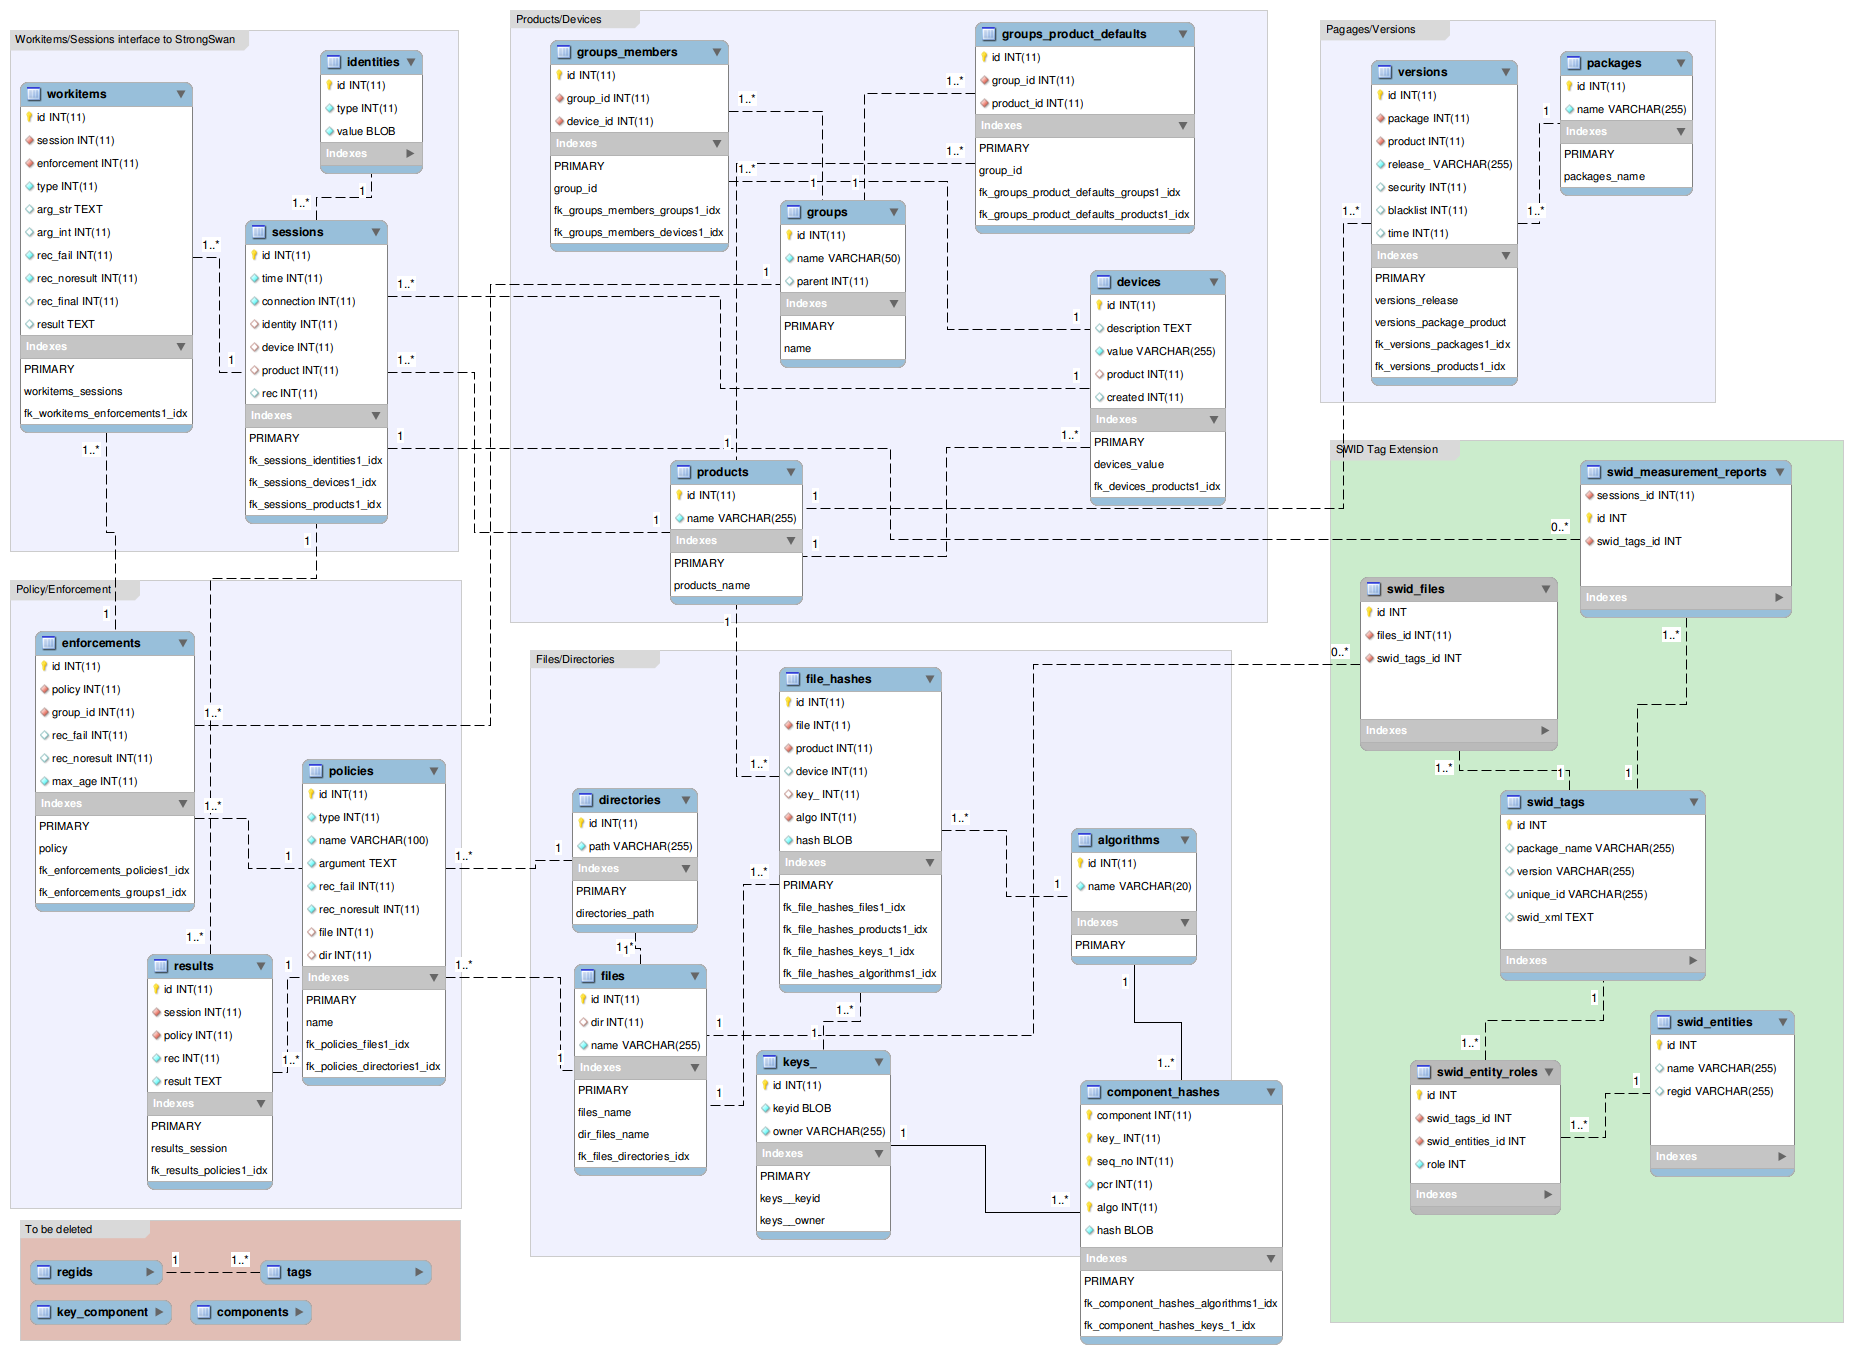
\includegraphics[angle=90,width=0.8\textwidth]{./images/db/database-model}
\caption{Bestehendes Datenmodel inklusive SWID Erweiterung (grün)}
\label{fig:database-model}
\end{figure}
Die Erweiterung des bestehenden Datenmodells ist in \autoref{fig:database-model} zu sehen. Die hinzugefügten Tabellen sind durch den grünen Hintergrund hervorgehoben. Bei Tabellen mit grauem Rahmen handelt es sich um Zwischentabellen, welche eine N zu M Beziehung auflösen. Beim modellieren der zusätzlichen Tabellen wurde darauf geachtet, dass keine bestehenden Tabellen angepasst werden mussten. Die Beziehungen werden daher alle von der Seite der Erweiterung hergestellt.
\begin{description}
\item [swid\_entityroles] Ein SWID Tag kann mehrere Entities enthalten. Entities haben nehmen in einem Tag eine oder eine Kombination von Rollen ein. Es existieren die Rollen Tag Creator, Licensor und Publisher. Pro SWID Tag darf es allerdings nur einen Tag Creator geben. Dieser Constraint wird jedoch erst in den Django Models durch das \gls{ORM} angewandt.

\item [swid\_tags\_files] In dieser Tabelle wird die Beziehung zwischen einem File und einem SWID Tag festgehalten. Ein SWID Tag kann mehrere Files beinhalten (\nameref{strongTNC:UC04}).

\item[swid\_tags\_sessions] Beim Durchführen einer Messung von SWID Tags werden die entsprechenden Tags in dieser Tabelle abgespeichert (\nameref{strongTNC:UC06}). Im dieser Tabelle werden die gemessenen Tags mit passenden Session verknüpft.

\item[swid\_entity] 
Diese Tabelle beinhaltet alle erfassten Entities. In der Regel ist eine kleine Anzahl unterschiedlicher Entities zu erwarten, weshalb diese in einer eigenen Tabelle gehalten werden und über die swid\_entityroles mit den SWID Tags verknüpft werden.

\end{description}

\section{Architektur SWID Messung}
\begin{figure}[H]
\centering
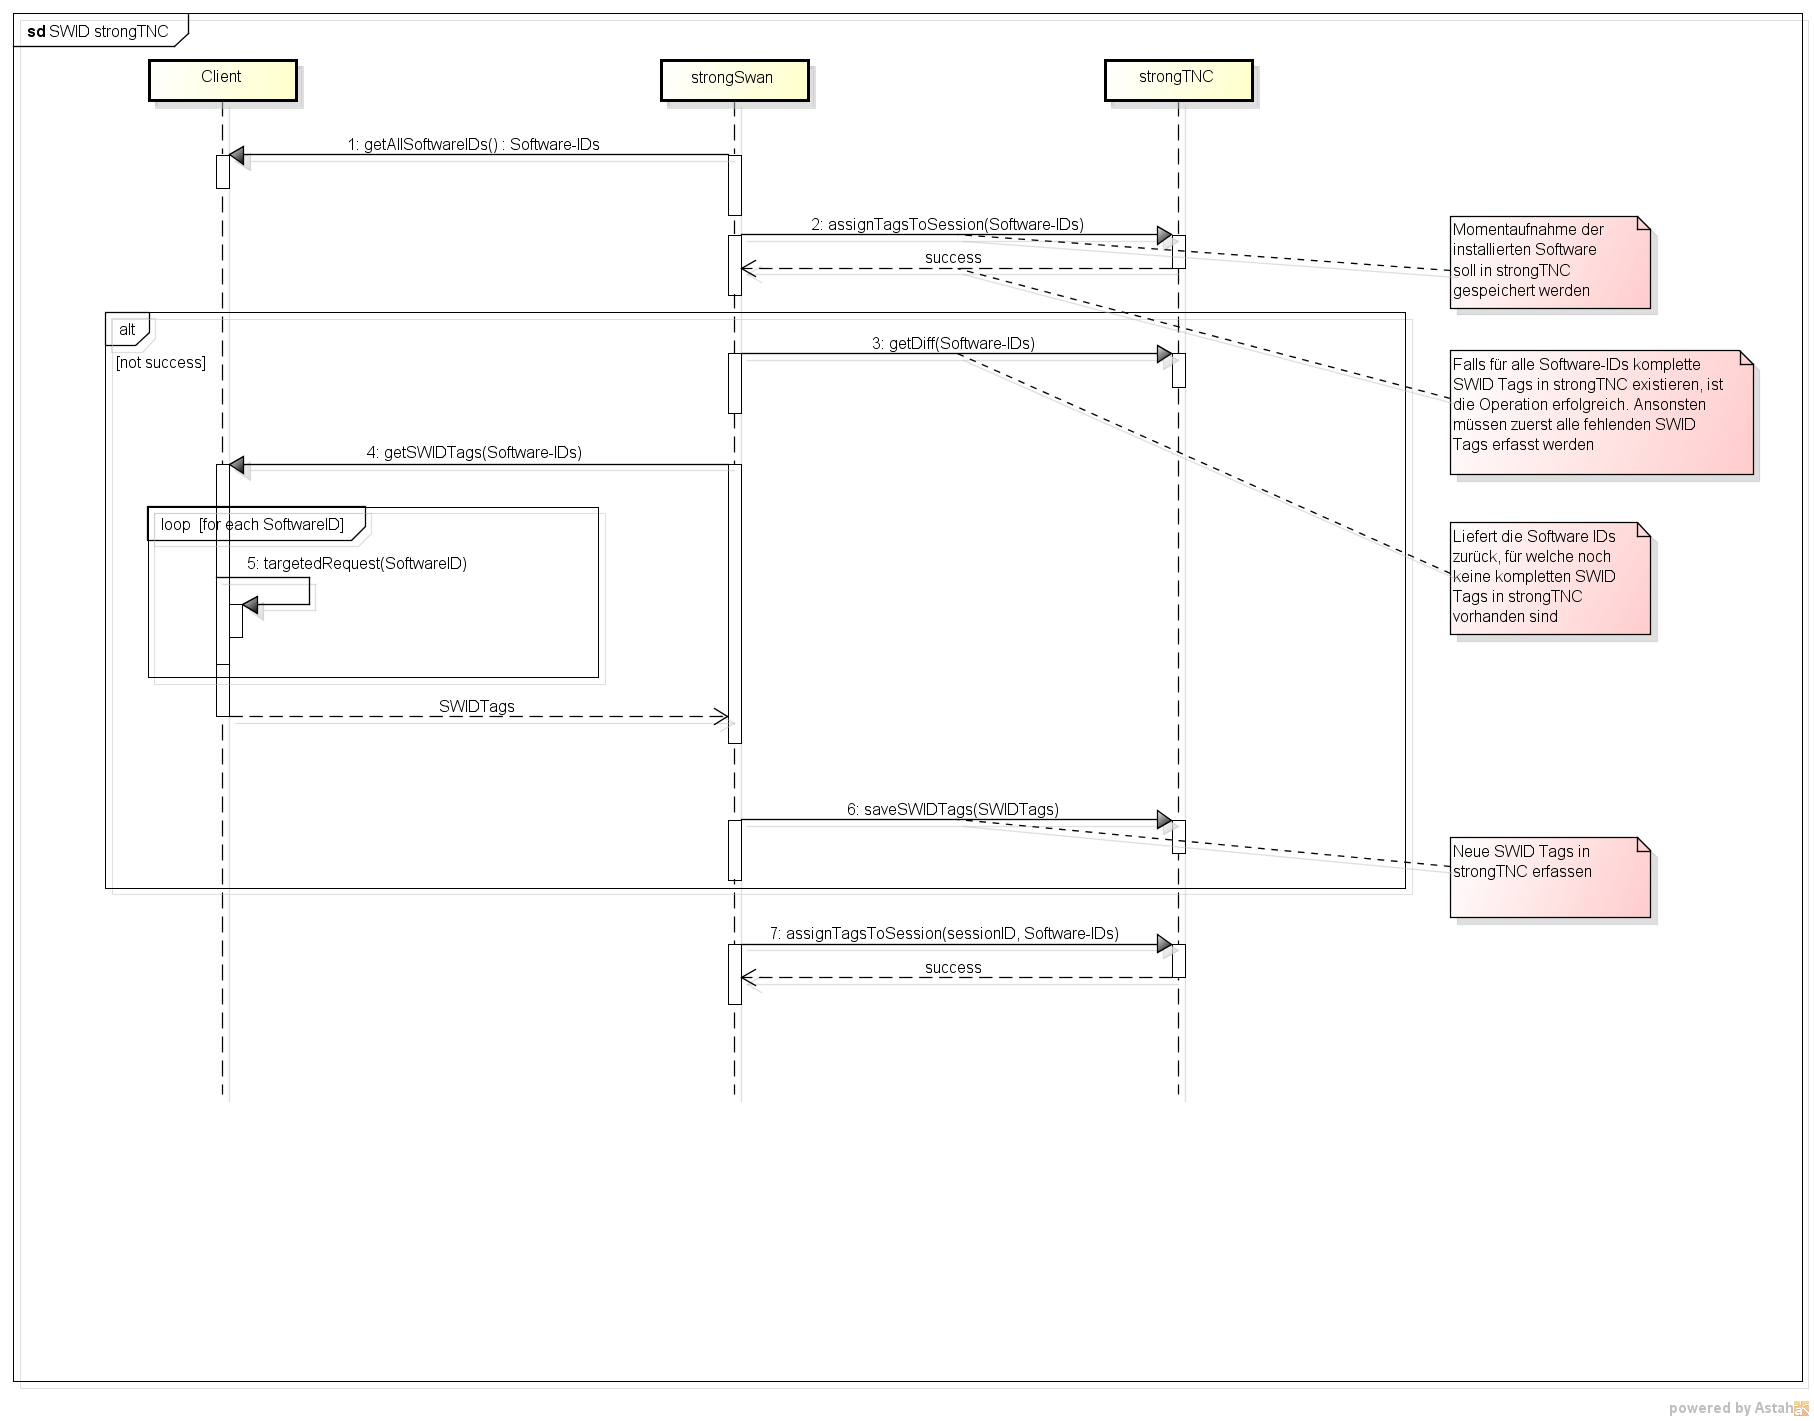
\includegraphics[width=0.9\textwidth]{./images/architecture/SWID_strongTNC.png}
\caption{Ablauf SWID Tag Messung eines Gerätes}
\label{fig:swid-measurement}
\end{figure}
In \autoref{fig:swid-measurement} ist der Ablauf der SWID Tag Messung (\nameref{strongTNC:UC06}) ersichtlich.
Eine Messung läuft wie folgt ab:
\begin{enumerate}
\item Auf dem Client werden die Software-IDs aller installierten Pakete generiert. 
\item Es wird versucht die Liste der generierten Software-IDs mit einer Session zu verknüpfen.
	\begin{itemize}
	\item Existiert zu allen Software-IDs ein entsprechender SWID Tag, ist die Messung abgeschlossen und die SWID Tags sind mit der Session verknüpft. ENDE
	\item Existiert für mindestens eine Software-ID kein entsprechender SWID Tag, wird die Messung abgebrochen und eine Liste jener Software-IDs, für welche kein SWID Tag existiert, zurückgeliefert. Weiter zu Punkt 3.
	\end{itemize}
\item Bevor die Messung durchgeführt werden kann, müssen die fehlenden SWID Tags erfasst werden. Die einzelnen XML Dokumente der SWID Tags werden vom Client anhand sogenannter \enquote{Targeted Requests} (TODO Referenz swidgenerator) erstellt, das heisst, der Generator kreiert gezielt die Tags für die gegebenen Software-IDs und nicht für alle installierten Software Pakete.
\item Der Client erfasst alle neu generierten SWID Tags in strongTNC.
\item Der Client startet erneut eine Messung und übermittelt nochmals alle Software-IDs. Nun sind für alle Software-IDs die entsprechenden SWID Tags vorhanden und die Messung wird erfolgreich abgeschlossen. Ansonsten weiter zu Schritt 2.
\end{enumerate}
Dieses Vorgehen erzwingt eine Aktualisierung der strongTNC Datenbank wenn diese nicht alle SWID Tags enthält, bevor eine Messung erfolgreich abgeschlossen werden kann. Dadurch wird erreicht, dass auf Serverseite kein Zustand gewahrt werden muss, wie es für eine nicht abgeschlossene Messung, welche später abgeschlossen wird, der Fall wäre. Dieses Vorgehen entspricht den Prinzipien von HTTP, eine Messung kann jederzeit durchgeführt werden ohne das ein Zustand oder Kontextinformationen vorhanden sein müssen. Das heisst, wenn eine Messung nicht vollständig und korrekt durchgeführt werden kann, werden keine Daten verändert. 



\subsection{Technische Umsetzung}
Der Zugriff auf die beschriebene Systemoperation erfolgt durch die, in dieser Arbeit ausgearbeiteten, RESTful HTTP Schnittstelle. Das komplette Konzept ist in (TODO Referenz REST Konzept) zu finden.

\subsubsection{REST Kommunikation}
Im Folgenden soll der Ablauf einer Messung anhand eines konkreten Beispiels illustriert werden.
In diesem Beispiel soll eine Messung für 3 Tags mit folgenden Software-IDs erfolgen:
\begin{textcode}
regid.2004-03.org.strongswan Ubuntu 12.04-i686-logrotate-3.7.8-6ubuntu5
regid.2004-03.org.strongswan Ubuntu 12.04-i686-lsb-base-4.0-0ubuntu20
regid.2004-03.org.strongswan Ubuntu 12.04-i686-strongswan-4.5.2-1.5+deb7u3
\end{textcode}

Der HTTP/REST Endpunkt wurde wie folgt definiert:
\begin{mdframed}[style=def]
\begin{description*}
	\item[URI Path] \texttt{/products/}
	\item[Archetype] Collection
	\item[Methods] GET, POST
	\item[JSON Format Response] \hfill
	
\begin{jsoncode}
{"data" : 
	[
	"software-ids TODO vom api konzept kopieren!" 
	]
}
\end{jsoncode}
\end{description*}
\end{mdframed}



\subsubsection*{Übermitteln von Software-IDs}
Die Daten werden als JSON-Liste an den entsprechenden Endpoint gesendet.
Der HTTP Request sieht folgendermassen aus:

\begin{listing}
\caption{Übermitteln von Software-IDs via HTTP/REST API}
\begin{httpcode}
POST /api/sessions/2/swid-measurement/ HTTP/1.1
Authorization: Basic cm9vdDpyb290
Host: tncserver:8000
Accept: application/json
Content-Type: application/json; charset=utf-8
Content-Length: 232

{
	"data":
	[
		"regid.2004-03.org.strongswan_Ubuntu_12.04-i686-logrotate-3.7.8-6ubuntu5",
		"regid.2004-03.org.strongswan_Ubuntu_12.04-i686-lsb-base-4.0-0ubuntu20",
		"regid.2004-03.org.strongswan_Ubuntu_12.04-i686-strongswan-4.5.2-1.5+deb7u3"
	]
}
\end{httpcode}
\end{listing}

Der entsprechende CURL Befehl:

\begin{bashcode}
curl -i -X POST http://tncserver:8000/api/sessions/2/swid-measurement/ \
		 -u username:password \
		 -H "Accept: application/json" \
		 -H "Content-Type: application/json; charset=utf-8" \
		 -d "$DATA"
\end{bashcode}

\subsubsection*{Antwort - Status 412 Precondition Failed}

Sind noch nicht alle Tags in der strongTNC Datenbank vorhanden, werden die
Software-IDs der fehlenden Tags zurückgeliefert. Der HTTP Status Code ist
``\texttt{412 Precondition Failed}''. Es werden zu diesem Zeitpunkt noch keine
Tags mit der Session verknüpft. Eine entsprechende Antwort kann wie folgt
aussehen:

\begin{listing}
\caption{HTTP Response mit Status Code 412 PRECONDITION FAILED}
\begin{httpcode}
HTTP/1.0 412 PRECONDITION FAILED
Date: Wed, 14 May 2014 15:21:45 GMT
Server: WSGIServer/0.1 Python/2.7
Vary: Accept, Cookie
Content-Type: application/json
Allow: POST, OPTIONS

["regid.2004-03.org.strongswan_Ubuntu_12.04-i686-strongswan-4.5.2-1.5+deb7u3"]
\end{httpcode}
\end{listing}

\subsubsection*{Antwort - Status 200 OK}

Wären für alle Software-IDs bereits Tags in der Datenbank vorhanden, könnte die Antwort wie folgt aussehen:

\begin{listing}
\caption{HTTP Response mit Status Code 200 OK}
\begin{httpcode}
HTTP/1.0 200 OK
Date: Wed, 14 May 2014 15:21:45 GMT
Server: WSGIServer/0.1 Python/2.7
Vary: Accept, Cookie
Content-Type: application/json
Allow: POST, OPTIONS

[]
\end{httpcode}
\end{listing}

\subsubsection*{Nacherfassen von SWID Tags}
War die Messung nicht erfolgreich (HTTP 412), müssen für die zurückgelieferten Software-IDs
zuerst komplette SWID Tags erfasst werden. Die Daten für diesen Request bestehen aus einer JSON-Liste von XML Strings, dadurch können auch
mehrere Tags auf einmal erfasst werden. Empfehlenswert ist allerdings ein Batching in mehrere Gruppen, da die Requests sonst unter Umständen sehr lange
dauern können. 

\pagebreak
Der Request sieht folgendermassen aus:

\begin{listing}
\caption{SWID Tags erfassen via HTTP/REST API}
\begin{httpcode}
POST /api/swid/add-tags/ HTTP/1.1
Authorization: Basic cm9vdDpyb290
Host: tncserver:8000
Accept: application/json
Content-Type: application/json; charset="utf-8"
Content-Length: 239

{ "data" : 
	[
		"<?xml version=\"1.0\" encoding=\"utf-8\"?><SoftwareIdentity name=\"fortune-mod\"...",
		"<?xml version=\"1.0\" encoding=\"UTF-8\"?><SoftwareIdentity name=\"strongswan\"..."
	]
}

\end{httpcode}
\end{listing}

Curl Befehl:

\begin{bashcode}
curl -i -X POST http://tncserver:8000/api/swid/add-tags/ \
		 -u username:password \
		 -H "Accept: application/json" \
		 -H "Content-Type: application/json; charset=utf-8" \
		 -d "{ \"data\" : $DATA }"
\end{bashcode}

Eine ausführliche Spezifikation zur Kommunikation mit diesem REST Endpoint ist im Anhang \autoref{REST:swid-measurement-manual} zu finden.
Darin sind unter anderem noch weitere Informationen zu Fehlersituationen aufgeführt.

\subsection{SWID Views}
Für die SWID Tag Erweiterungen wurden drei zusätzliche Views implementiert.
\subsubsection{Regid View}
Der Zweck der Regid Ansicht ist das auflisten im System vorhandener Entitys (\nameref*{strongTNC:UC03}).
Beim wählen einer Entity werden die referenzierten Tags aufgelistet. 
\begin{figure}[H]
\centering
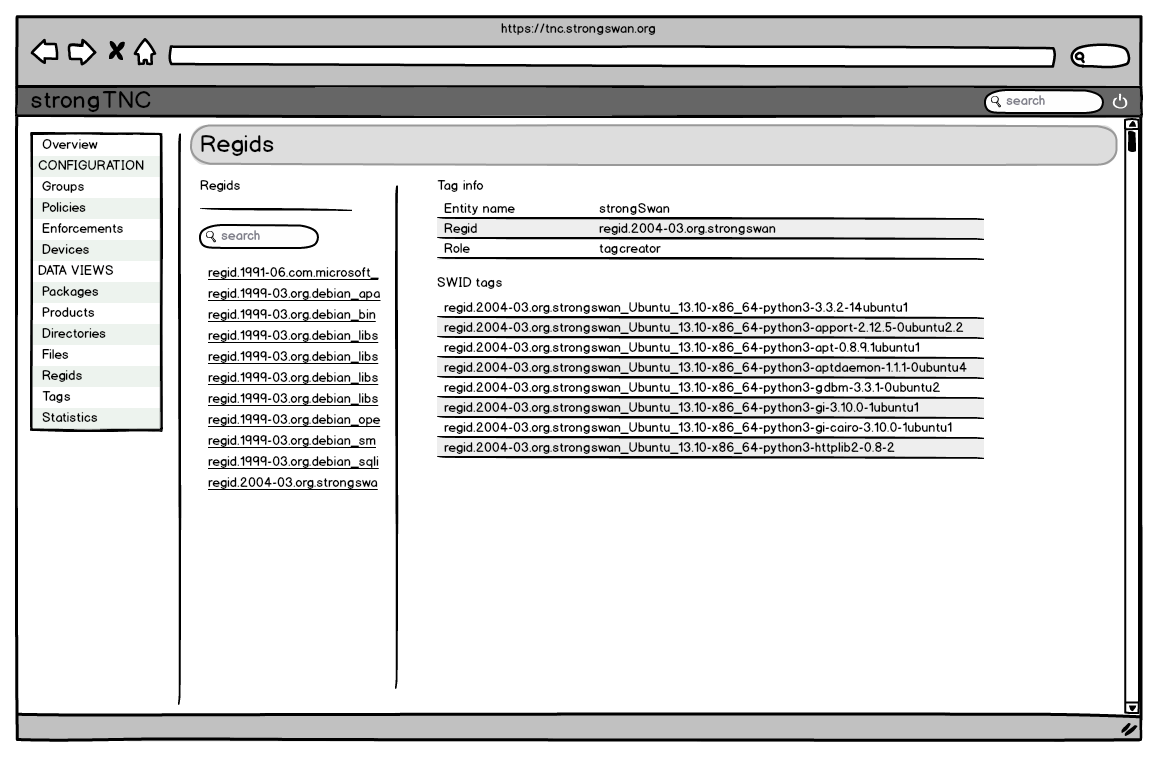
\includegraphics[width=0.8\textwidth]{./images/mockups/swid-regid-view}
\caption{Mockup Regid View.}
\label{fig:swid-regid-view}
\end{figure}
\begin{figure}[H]
\centering
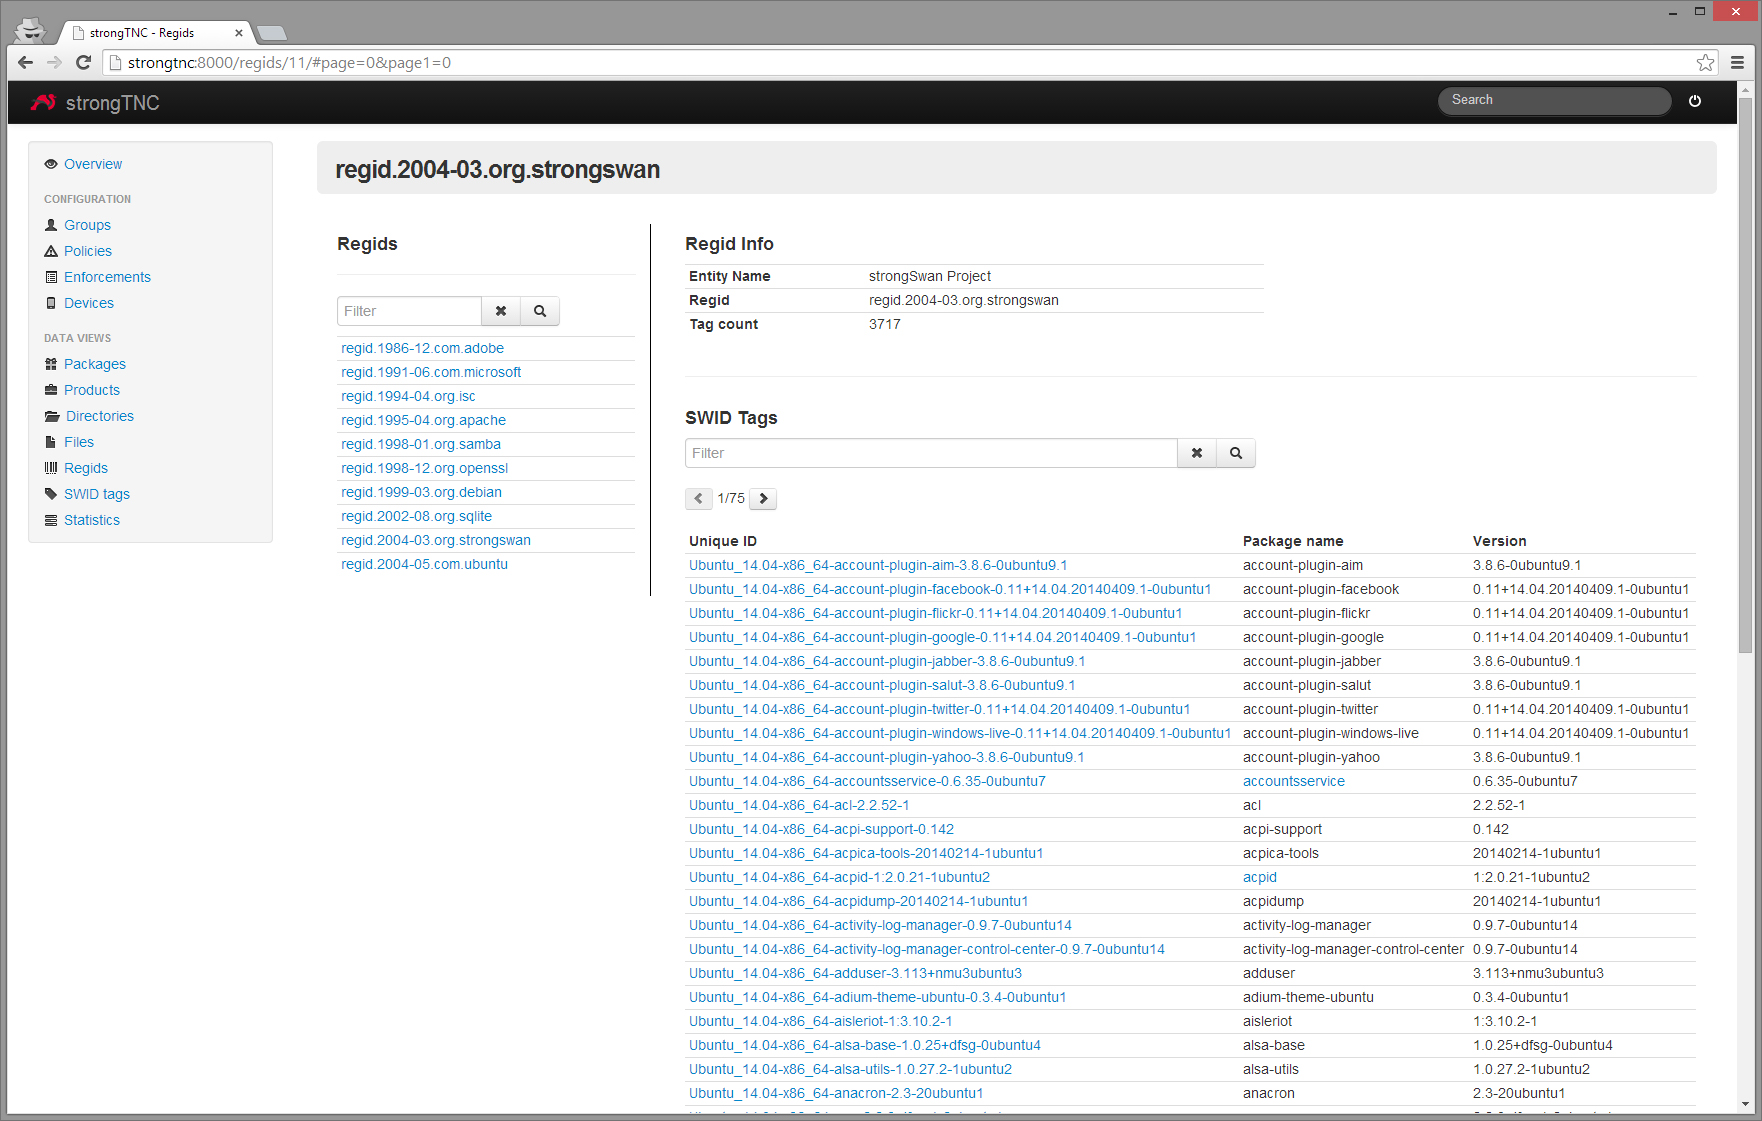
\includegraphics[width=0.8\textwidth]{./images/Views/regid-view}
\caption{Regid View mit Detailansicht}
\label{fig:regid-view}
\end{figure}

\subsubsection{SWID Tag View}
Der Zweck der SWID Tag Ansicht ist das Auflisten im System vorhandener SWID Tags (\nameref{strongTNC:UC04}).
Beim wählen eines SWID Tags werden Detailinformationen angezeigt.

\begin{figure}[H]
\centering
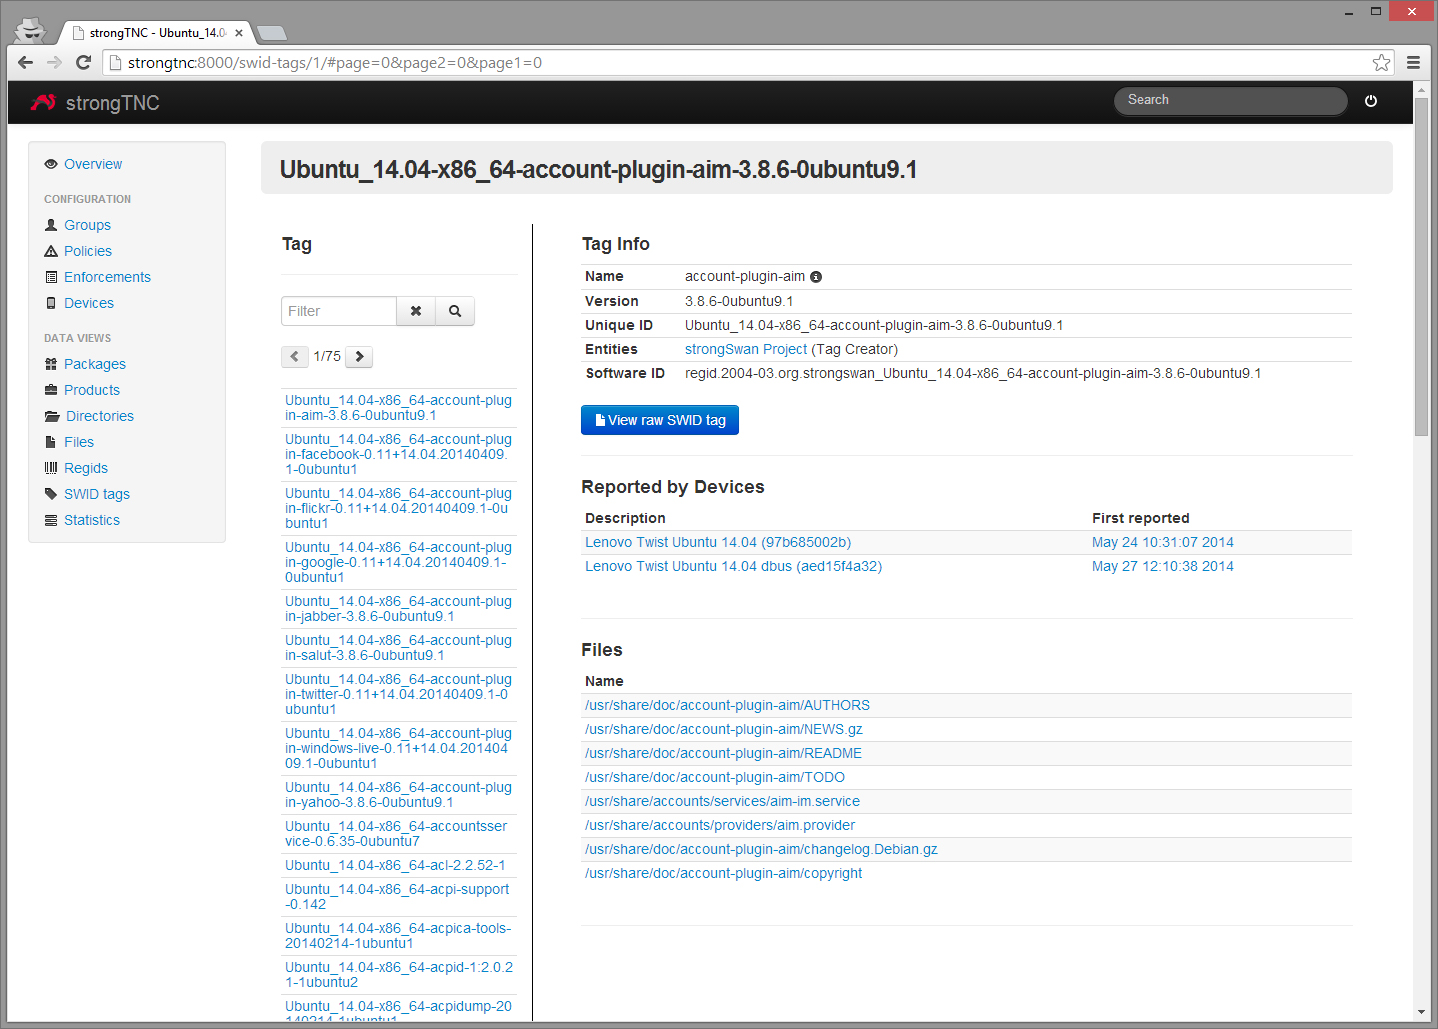
\includegraphics[width=0.8\textwidth]{./images/Views/tag-detail-view}
\caption{SWID Tag View mit Anzeige detaillierter Tag Informationen}
\label{fig:tag-detail-view}
\end{figure}

\subsubsection{SWID Inventory View}

Anhand der SWID Inventory View kann festgestellt werden, welche Software für eine ausgewählte Sitzung (Session) auf einem Gerät installiert war (\nameref{strongTNC:UC01}).

\begin{figure}[H]
\centering
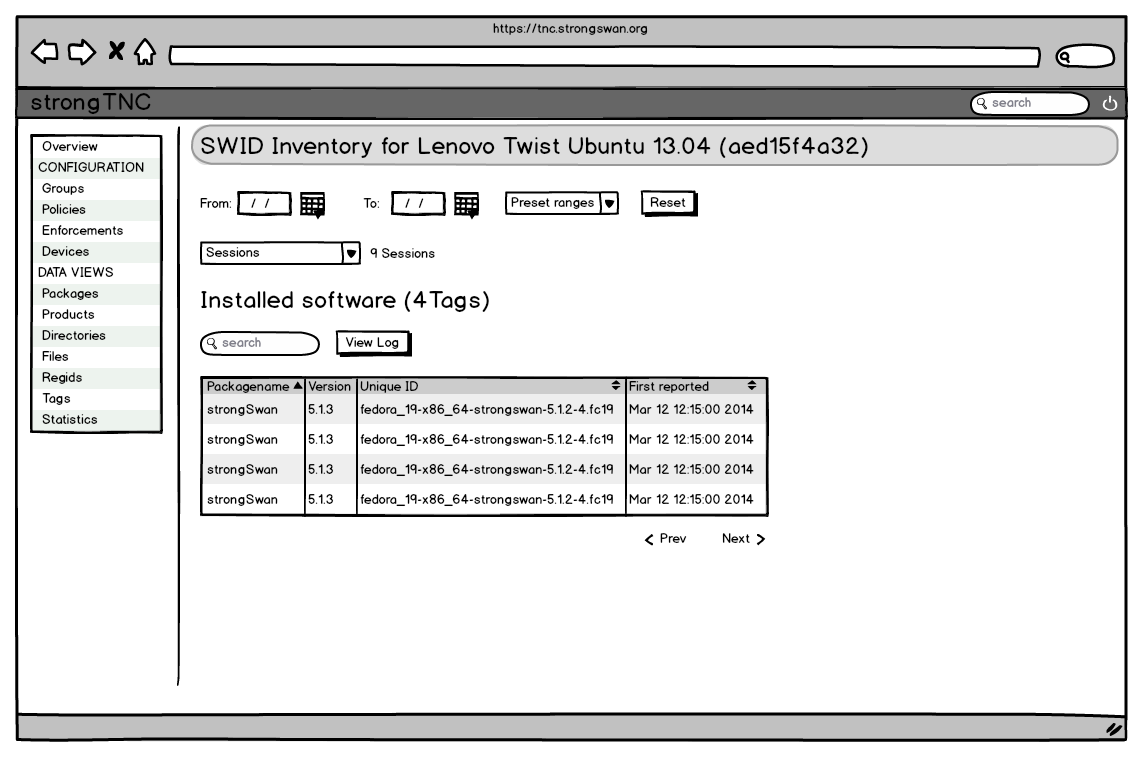
\includegraphics[width=0.8\textwidth]{./images/mockups/swid-inventory}
\caption{}
\label{fig:swid-inventory}
\end{figure}

\begin{figure}[H]
\centering
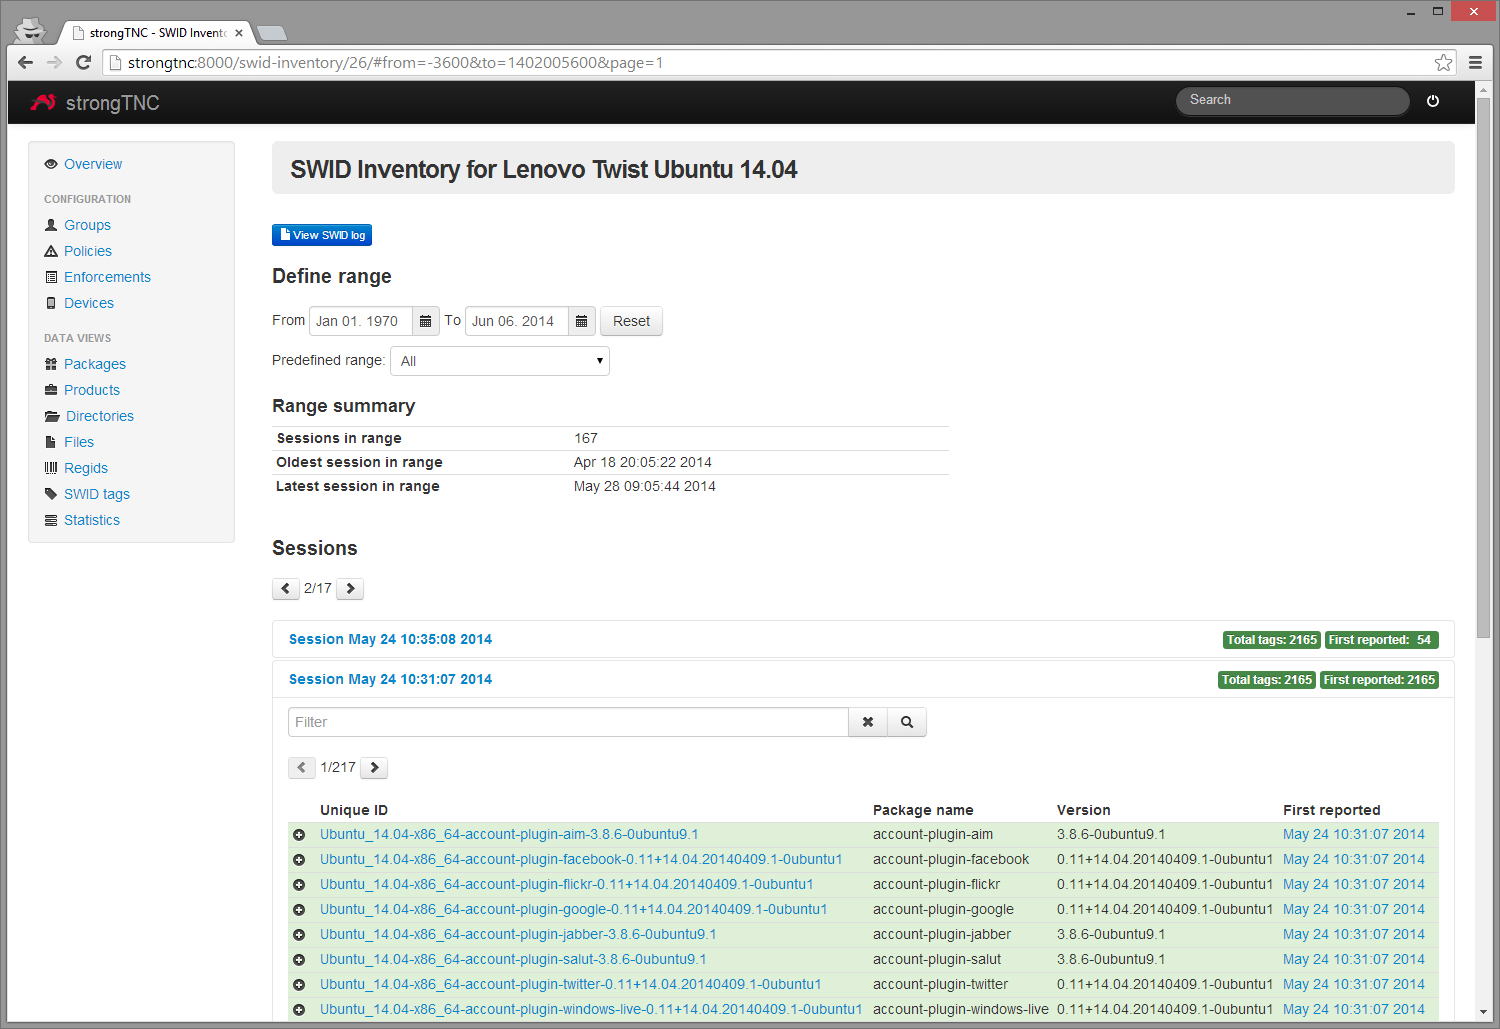
\includegraphics[width=0.8\textwidth]{./images/Views/inventory-view}
\caption{SWID Inventory View}
\label{fig:tag-detail-view}
\end{figure}


\subsubsection{SWID Log View}

Die Log View zeigt den Verlauf der Installation und Entfernung von Software Paketen auf
einem ausgewählten Gerät (\nameref{strongTNC:UC01}). Da bei jeder SWID Tag Messung jeweils alle
vorhanden SWID Tags übermittelt werden, lässt sich für jedes Paket sagen, wann
es installiert, beziehungsweise entfernt wurde. 

\begin{figure}[H]
\centering
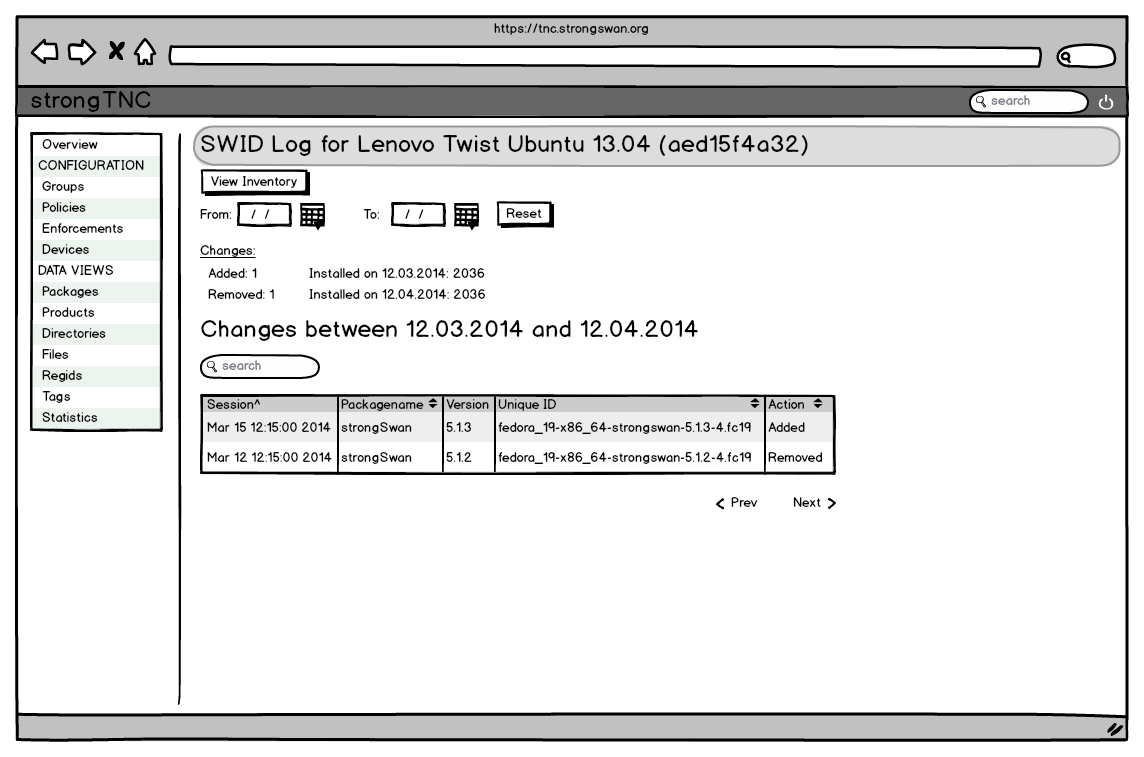
\includegraphics[width=0.8\textwidth]{./images/mockups/swid-log}
\caption{SWID Log View Mockup}
\label{fig:swid-log}
\end{figure}

\begin{figure}[H]
\centering
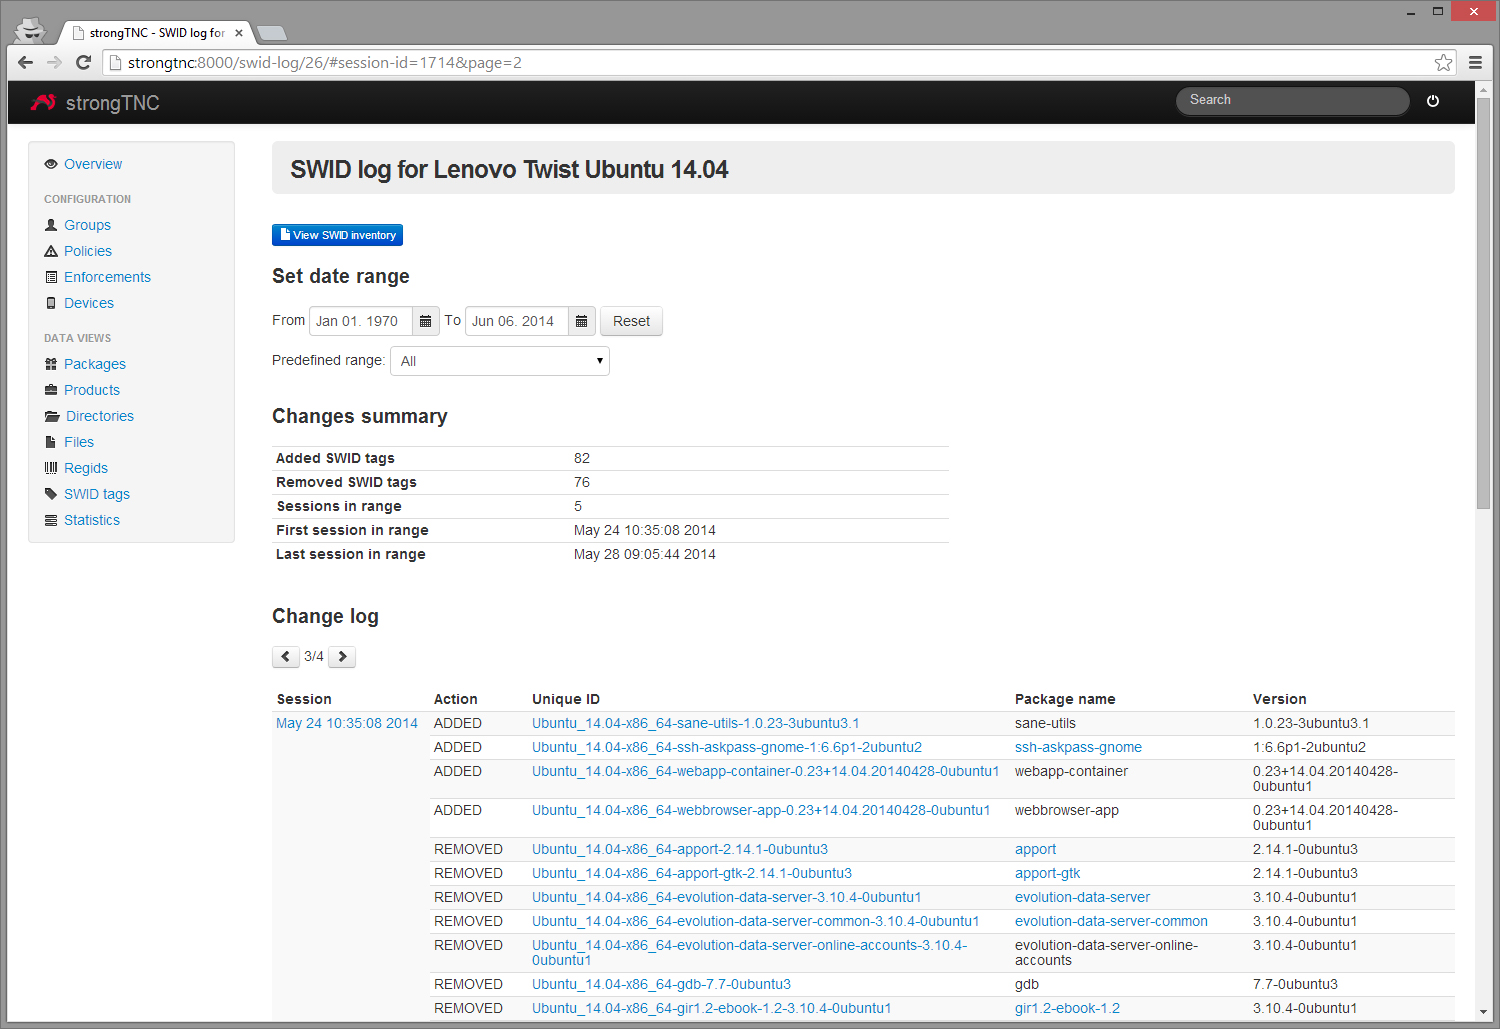
\includegraphics[width=0.8\textwidth]{./images/Views/log-view}
\caption{SWID Log View mit Details für eine ausgewählte Session}
\label{fig:log-view}
\end{figure}


\section{Verbesserungen}

\subsection{Multi-Rollen Konzept}

\subsubsection{Einleitung}

Um die Informationen in strongTNC zu Präsentationszwecken zugänglich machen zu können, 
ohne dass Änderungen vorgenommen werden können, weder absichtlich noch aus Versehen, 
soll eine Read-Only Rolle eingeführt werden.


\subsubsection{Ziel}
In einem ersten Schritt soll ein Rollen-Modell mit zwei Rollen eingeführt werden. 
Eine Rolle für Read-Only Zugriff und eine für den Vollzugriff. Der Zugriff soll, 
so wie es gegenwärtig implementiert ist, nicht personalisiert sein. Die Möglichkeit, 
den Login zu personalisieren sollte nicht grundsätzlich ausgeschlossen werden, jedoch 
steht die Implementation eines nicht personalisierten Read-Only Zugriffs im Vordergrund.


\subsubsection{Technische Umsetzung}

Django hat ein vollständiges Authentication- und Permission-System integriert. Damit 
lassen sich komplexe Permission-Szenarien abbilden, jedoch besteht auch die Möglichkeit 
nur Teile daraus zu verwenden und so ein einfacheres Rollen-Modell zu simulieren.

\paragraph*{User / Permissions}

Wenn keine personalisierten Login erwünscht sind, werden zwei technische User
erstellt, die für die beiden Rollen stehen. Das heisst es gibt beispielsweise
einen User \texttt{admin-user} und einen User \texttt{readonly-user}. Dem
\texttt{admin-user} wird die Permission \texttt{write\_access} erteilt, diese
Permission kann dann mittels \texttt{@permission\_required()} Decorator geprüft
werden.

Diese Umsetzungsvariante erlaubt es mit sehr wenig Aufwand personaliserte Logins
einzuführen. Für die Verwaltung der User stellt Django ein Admin-Interface zur
Verfügung, dieses müsste also nicht selber entwickelt werden.

\paragraph*{Templates}

In den Templates können die Permissions über das perms Objekt im Context geprüft werden. 
Beispiel:

\begin{pythoncode}

    <p>Read-write access.</p>

\end{pythoncode}

\paragraph*{Alternativen}

Als Alternative zum Permission-System könnten auch die standardmässig vorhandenen Flags 
\texttt{user.is\_admin} und \texttt{user.is\_staff} verwendet werden. Dies wäre bedeutend 
einfacher zu implementieren, die Lösung ist jedoch nicht ausbaufähig. Deshalb wird das 
Permission-System bevorzugt.


\subsubsection{Frontend Änderungen}
Folgende Änderungen müssen im User Interface vorgenommen werden.

\paragraph*{Login Screen}

Es muss eine Auswahl für die gewünschte Rolle zur Verfügung stehen. Diese kann bei zwei fix 
definierten Gruppen als Dropdown realisiert werden. Optional kann auch ein Inputfeld mit einem 
Username verwendet werden. 

\begin{figure}[H]
	\centering
	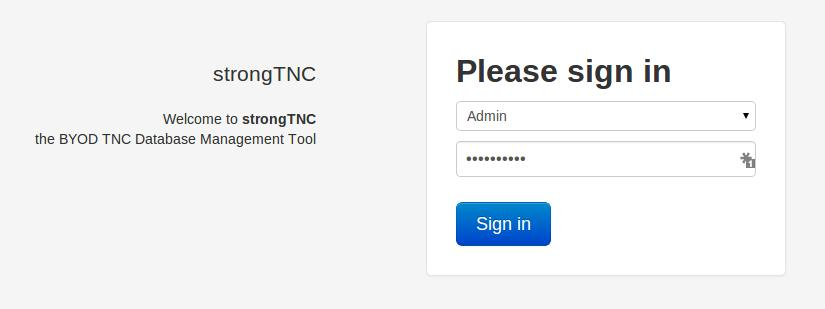
\includegraphics[width=\textwidth]{images/rollen-konzept/login-admin.jpg}
	\caption{Mögliches Aussehen der Loginmaske für den Adminlogin}
\end{figure}

\begin{figure}[H]
	\centering
	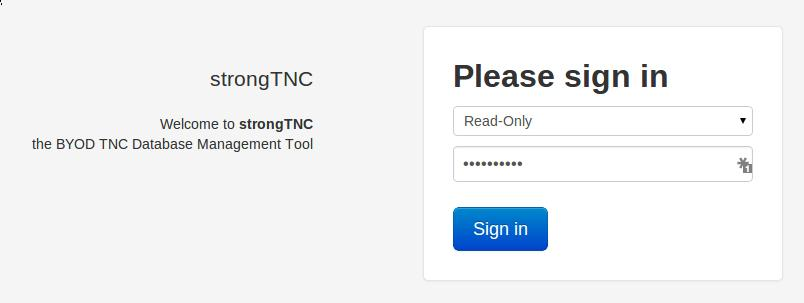
\includegraphics[width=\textwidth]{images/rollen-konzept/login-read-only.jpg}
	\caption{Mögliches Aussehen der Loginmaske für den Read-Only-Zugriff}
\end{figure}

\subsubsection{Configuration- und Data-Templates}

Alle Form-Elemente die einen Input erlauben werden deaktiviert, dies kann durch das 
Hinzufügen des HTML-Attribut \text2tt{disabled} erreicht werden. Alle Buttons werden entfernt.

\paragraph{Ausnahmen} \hspace{0pt} \\
\begin{itemize}
    \item In allen Views, das Filter-Feld
    \item In der Device-View, der Button "View device report"
\end{itemize}

\begin{figure}[H]
	\centering
	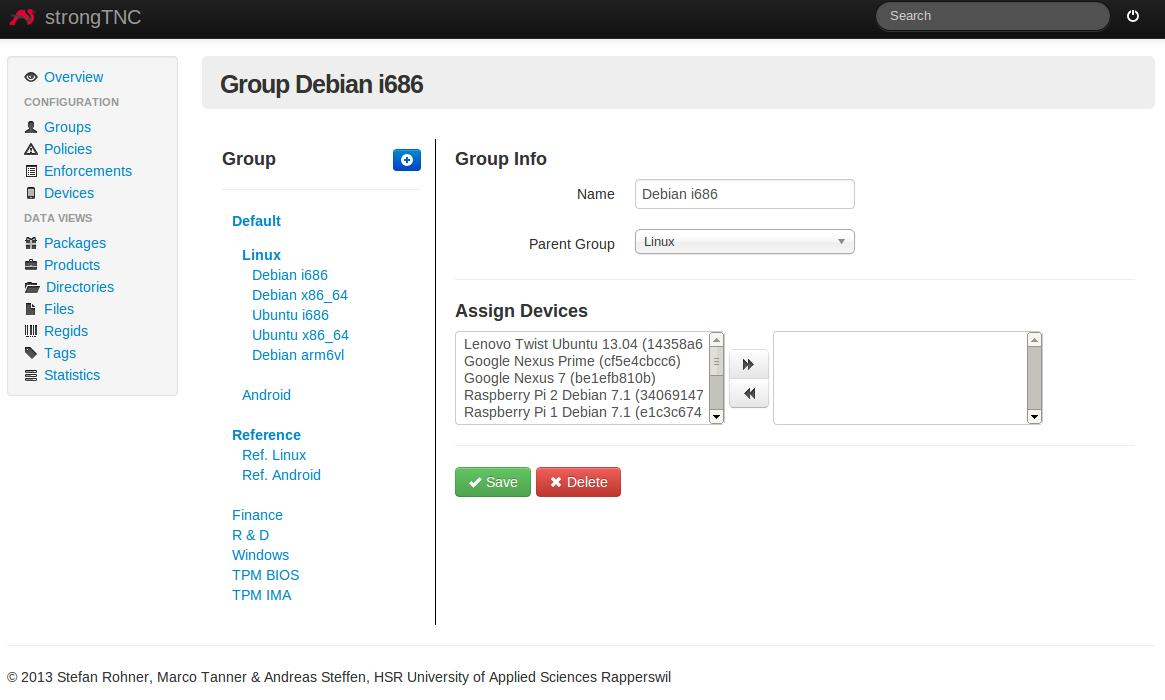
\includegraphics[width=\textwidth]{images/rollen-konzept/group-view-admin.jpg}
	\caption{Mögliches Aussehen der einer View für den Vollzugriff, am Beispiel der aktuellen Group-View}
\end{figure}

\begin{figure}[H]
	\centering
	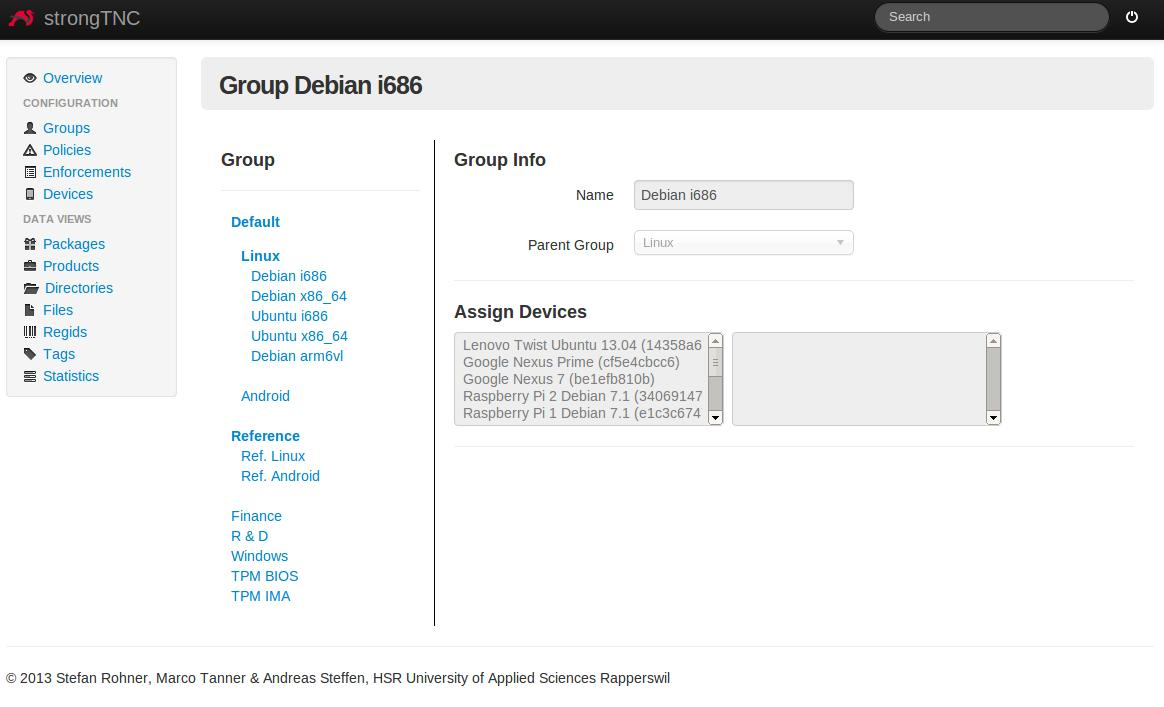
\includegraphics[width=\textwidth]{images/rollen-konzept/group-view-read-only.jpg}
	\caption{Mögliches Aussehen der einer View für den Read-Only Zugriff, am Beispiel der aktuellen Group-View}
\end{figure}


\subsubsection{Backend Änderungen}

Die meisten Views sind sehr ähnlich aufgebaut und verfügen über die gleichen Grundfunktionen, 
diese sind wie folgt einzuschränken:

\begin{description}
    \item [\texttt{models}] Nicht eingeschränkt
    \item [\texttt{model}] Nicht eingeschränkt
    \item [\texttt{add}] Eingeschränkt, nur für Admin
    \item [\texttt{save}] Eingeschränkt, nur für Admin
    \item [\texttt{delete}] Eingeschränkt, nur für Admin
    \item [\texttt{search}] Nicht eingeschränkt
    \item [\texttt{check}] Eingeschränkt, nur für Admin
\end{description}

Mit \texttt{models}, bzw. \texttt{models} sind die Funktionen einer View gemeint, die jeweils mit dem
Namen des Models benannt sind, zum Beispiel in der View \texttt{policy\_views.py}, die Funktionen
\texttt{policy()} und \texttt{policies()}.

\paragraph{Ausnahmen} \hspace{0pt} \\

\textbf{Device View:}
\begin{description}
    \item [\texttt{report} ] Nicht eingeschränkt
    \item [\texttt{session} ] Nicht eingeschränkt
\end{description}

\textbf{Package View:}
\begin{description}
    \item [\texttt{toggle\_version}] Eingeschränkt, nur für Admin
\end{description}



\section{Trennung, API Konzept}

